\section{Quantification}

As mentioned in \cref{sec:crna_quantification}, all the \gls{bsj} detection
tools also quantify the number of reads supporting each \gls{bsj}.
However, there are several tools that focus on the quantification of
\gls{crna}s based on previously detected \gls{bsj}s.
nf-core/circrna offers two such tools: CIRIquant and psirc-quant.

Due to the lack of a ground truth or a gold standard, the quantification
results were compared to each other.
The correlation heatmap in \cref{fig:quantification_correlation_heatmap} shows
the Pearson correlation coefficient between the quantification results of the
detection tools, multiple aggregations of the detection tools, and the
quantification tools.

\begin{figure}[ht]
    \centering

    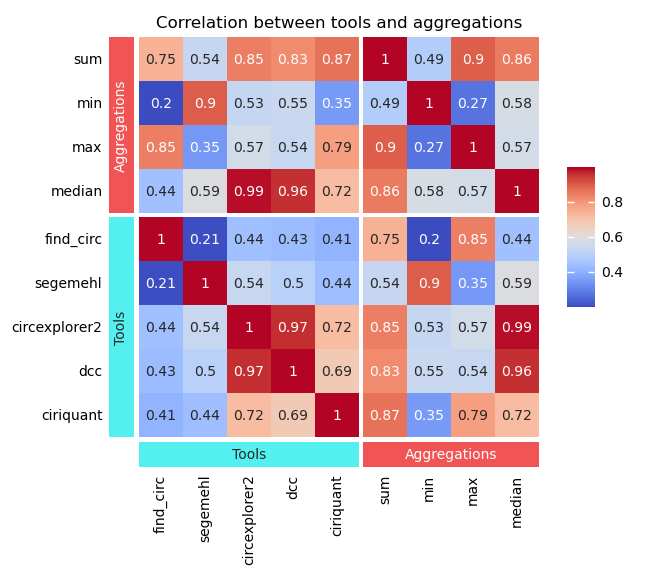
\includegraphics[width=0.7\textwidth]{chapters/4_results_and_discussion/figures/quantification/correlation_heatmap.png}
    \caption{Pearson correlation heatmap between the quantification results of
        the
        detection tools, multiple aggregations of the detection tools, and the
        quantification tools.
        A maximum shift of 1 was used to cluster close \gls{bsj}s.
        If a certain detection or quantification tool did not detect any candidate for
        a specific cluster, it was inferred to have a value of 0.
    }
    \label{fig:quantification_correlation_heatmap} \end{figure}

With the exception of Segemehl, all detection tools show a correlation of at
least 0.5.
The highest correlation among the detection is observed between CircExplorer2
and DCC, with a Pearson correlation coefficient of 0.97.

When looking at the aggregations, Segemehl shows a high correlation of 0.9 with
the minimum of all tools, indicating that it usually among the tools with the
lowest number of reads supporting a \gls{bsj}.
Other than this, the sum and median aggregations show 

While both these tools showed great performance in their respective
publications,
